\section{Introduction}
\label{sec:intro}

All-day wearable AR glasses promise to be the next big paradigm shift in computing: They can lift interaction with the digital world from 2D screens into the 3D world around us; blending seamlessly into our lives as opposed to diverting our attention into small 2D rectangles held in our hands. Yet, in order to be more than mere 3D versions of 2D screens, they also require a new compute- and interaction-paradigm that is context-aware, highly personalized and natural to interact with. Creating this new paradigm is a significant challenge that still requires a broad range of research to be solved.
%
Fortunately, the recent breakthrough of internet-trained Large Language Models such as GPT4~\cite{openai2023gpt4} and llama2 \cite{touvron2023llama} promise to solve a major part of this challenge, making it a lot more tractable:
They demonstrate that modern Transformer architectures combined with sufficient training data enable both long-range reasoning and information retrieval while also adopting seamlessly to new tasks using a local context window and prompt engineering. Taken together, this enables human-level interaction with digital agents that blend into how we humans interact naturally. 

\begin{figure}
    \centering
    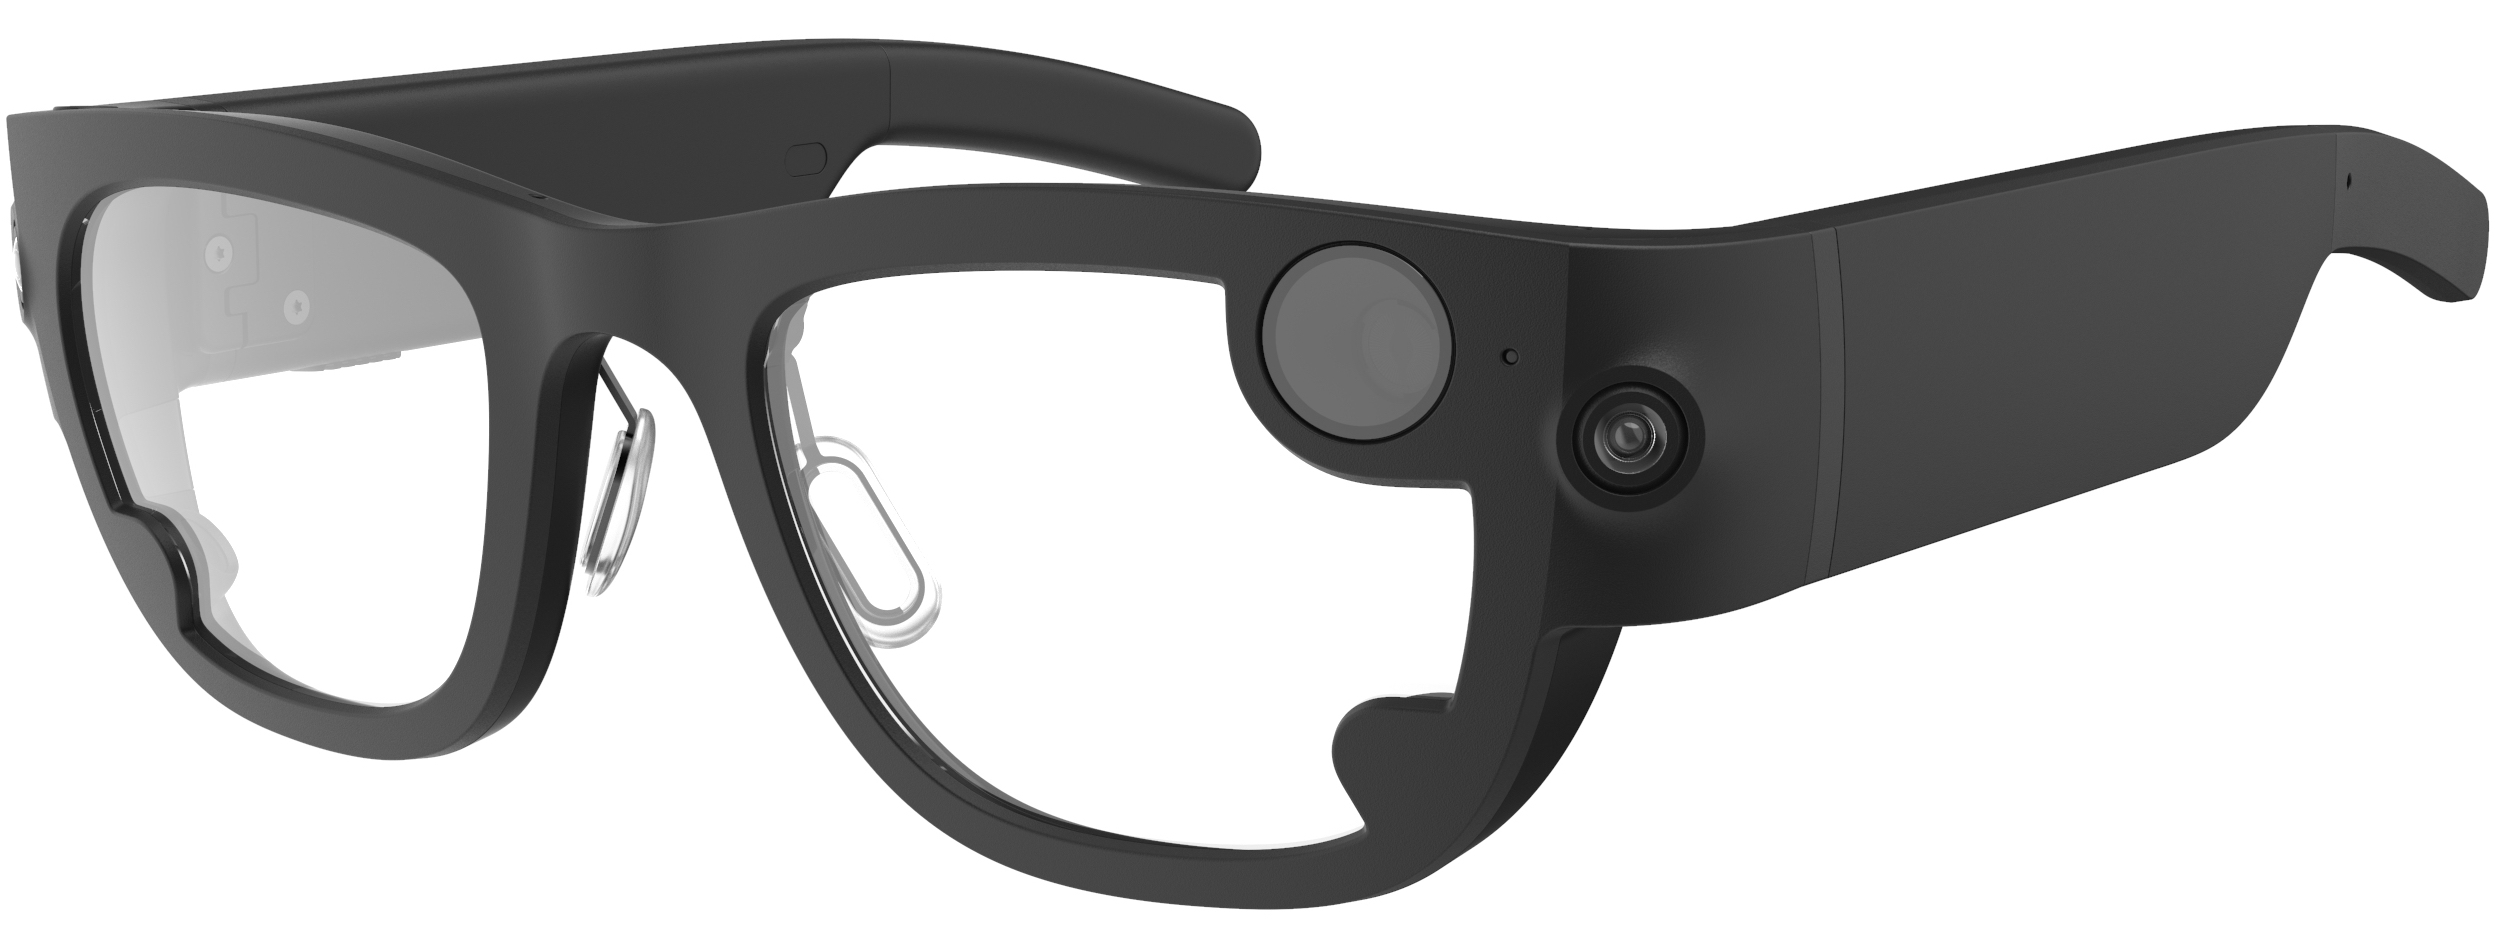
\includegraphics[width=\linewidth]{images/sensors_aria_plain_cropped.jpg}
    \caption{The \AriaDevice.}
    \label{fig:aria-image}
\end{figure}
\subsection{\ProjectAria}

However, we believe that this paradigm shift in personalized computing requires another crucial ingredient: the ability for AI Agents to adapt to the unique, personal context and preferences of the \textit{individual user}. Some of this can be achieved by leveraging a persons digital footprint -- the aggregate of interactions with the internet through phones and laptops. It is only a matter of time for such personalized AI Assistants to emerge. Yet, our digital footprint only represents a small fraction of the experiences that matter to us, and rarely contain the most important ones, which play out in the real world, are highly personal and often take place in unpredictable places and at unpredictable times. 

Importantly, this applies not only on an individual level, but also in aggregate: The wealth of digital data accumulated over 25 years in the digital realm only represents a small -- and often severely biased -- fraction of the sum total of human experience. For example, the overwhelming majority of images available on the web and used to train AI models were consciously captured with handheld devices and curated before upload. Any outtakes, any data that is not deemed interesting is typically deleted or edited although it arguably represents the majority of situations we encounter in our daily life.

A direct consequence of this is that many state of the art methods in the space of Machine Perception and AI (DALL·E2\cite{ramesh2022hierarchical}, GPT-4~\cite{openai2023gpt4}, DreamFusion~\cite{poole2022dreamfusion}, SAM~\cite{kirillov2023segment}, MaskRCNN~\cite{he2017mask}, CLIP~\cite{radford2021learning}, DINOv2~\cite{oquab2023dinov2}) excel when applied to allocentric 2D images and viewpoints, but fare comparatively poorly at tasks that involve egocentric data or require structured reasoning and understanding in 3D/4D space. While  this is partially due to the increase in data/compute requirements, it is also a direct result of the aforementioned shortcomings of data typically  
available through web platforms.

In order to address this gap and to enable the next big paradigm shift towards context-aware, personalized, and human-oriented AI, we have created \textit{\ProjectAria}: At its core, the \AriaDevice{} is a data-capture system in glasses form factor that is sufficiently light and unobtrusive to be worn for long time-spans without inhibiting natural activities and behavior (see Figure~\ref{fig:aria-image}), allowing to capture \textit{ecologically valid} data. The device features a rich multi-modal sensor suite that approximates what can be expected in future AR glasses for the purpose of environment- and user-understanding. The onboard battery allows the device to record 1-2 hours of data (with the nominal recording profile). Much longer recordings are possible with an external power bank.

In this technical report, we introduce the \AriaDevice{} as well as the software and Machine Perception Services that come with it. We make these available to research institutions around the world to foster advancements in the field of egocentric perception towards personalized AI. 
We also summarize the principles and standards that we have established and adopted to protect the privacy of both wearers and bystanders in accordance with Meta's Responsible Innovation Principles \cite{metari}.

Since its launch in 2020, \AriaDevices{} have been used by research groups in the USA, UK, Switzerland, India, Canada, Singapore, Colombia and Japan. In 2022, we released the Aria Pilot Dataset~\cite{ariapilot}. 
To find out more about \ProjectAria{} and how to become a research partner, please visit our website~\cite{ariawebsite}.

This report is organized as follows: Section \ref{sec:device} introduces the \AriaDevice{} and its capabilities. Section \ref{sec:recordingtools} introduces the software and tools required for recording and using recordings for research. Section \ref{sec:mps} enumerates the set of first-level machine perception capabilities we offer through a web service in order to accelerate and simplify use of \ProjectAria{} data. Section \ref{sec:privacy} details the privacy and responsible innovation principles we have established, and how the \AriaDevice{} implements them. Section \ref{sec:applications} gives a set of example research applications that are enabled by Project Aria. We end this paper with a conclusion in Section \ref{sec:conclusion}.
